\begin{figure}[t]
    \begin{subfigure}[c]{0.3\textwidth}
        \begin{flushright}
        \vspace*{.4cm}
        Initial Image
        
        \vspace{1.3cm}
        
        CVQVAE (Ours)
        
        \vspace{1.3cm}
        
        CCVAE
        
        \vspace{0.35cm}
        \end{flushright}
    \end{subfigure}
    \begin{subfigure}[c]{0.3\textwidth}
        \scalebox{1.8}{
            \includegraphics[width=0.2\textwidth]{val/imgs/samples/real_new/s1.png} 
            % \hspace{-12px}
            \includegraphics[width=0.2\textwidth]{val/imgs/samples/real_new/s2.png}
            % \hspace{-12px}
            \includegraphics[width=0.2\textwidth]{val/imgs/samples/real_new/s3.png}
            % \hspace{-12px}
            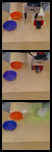
\includegraphics[width=0.2\textwidth]{val/imgs/samples/real_new/s4.png}
            % \hspace{-12px}
            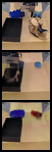
\includegraphics[width=0.2\textwidth]{val/imgs/samples/real_new/s5.png}
            % \hspace{-12px}
        }
    \end{subfigure}
    % \begin{subfigure}[b]{0.3\textwidth}
    %     \scalebox{1.45}{
    %             \adjustbox{trim=0 16 0 0,clip} { \includegraphics[width=0.1\textwidth]{imgs/samples/real/s1.png} } \hspace{-12px}
    %             \adjustbox{trim=0 16 0 0,clip} { \includegraphics[width=0.1\textwidth]{imgs/samples/real/s2.png} } \hspace{-12px}
    %             \adjustbox{trim=0 16 0 0,clip} { \includegraphics[width=0.1\textwidth]{imgs/samples/real/s3.png} } \hspace{-12px}
    %             \adjustbox{trim=0 16 0 0,clip} { 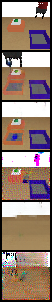
\includegraphics[width=0.1\textwidth]{imgs/samples/real/s4.png} } \hspace{-12px}
    %             \adjustbox{trim=0 16 0 0,clip} { 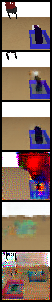
\includegraphics[width=0.1\textwidth]{imgs/samples/real/f1.png} } \hspace{-12px}
    %             \adjustbox{trim=0 16 0 0,clip} { \includegraphics[width=0.1\textwidth]{imgs/samples/real/14s.png} } \hspace{-12px}
    %         }
    % \end{subfigure}

    \caption{Samples on unseen objects in the real world. In each column, the top image is the conditioning image $s_0$ and the images below are conditionally sampled images from the corresponding generative model. Our model, CVQVAE, generates clear and diverse samples.}
    \label{fig:real_samples}
    %\vspace{-0.5cm}
\end{figure}